\documentclass[12pt, dvipsnames]{beamer}

\def\languages{french, english}

%%%%%%%%%%%%%%%%%%% Theme

\usetheme{metropolis}

%%%%%%%%%%%%%%%%%%% Libraries

\input{include/libraries/default.tex}
\input{include/libraries/figures.tex}
\input{include/libraries/mathematics.tex}
\input{include/libraries/units.tex}

%%%%%%%%%%%%%%%%%%% Additional packages

\usepackage{colortbl}
\usepackage{listings}

%%%%%%%%%%%%%%%%%%% Titlepage

\title{Computer Vision}
\subtitle{Project part 2}
\author{{\bf Team 4}\\M. Meurisse, F. Rozet, O. Rumfels and V. Vermeylen}
\institute{University of Liège}
\date{December 20, 2019}
\titlelogo{resources/pdf/logo-uliege.pdf}
\framelogo{resources/pdf/logo-uliege.pdf}

%%%%%%%%%%%%%%%%%%% Table of contents and footers

\setbeamertemplate{section in toc}[sections numbered]
%\setbeamertemplate{frame footer}{}

%%%%%%%%%%%%%%%%%%%

\begin{document}

% ----- Title ----- %
\maketitle

% ----- Introduction ----- %
\begin{frame}{Introduction}
    Divided into 2 parts :
    \begin{enumerate}
        \item Performance assessment of our line detection algorithms
        \item Digits recognition in sudoku grids
    \end{enumerate}
\end{frame}

% ----- Plan of the presentation ----- %
\begin{frame}{Plan of the presentation}
    \tableofcontents
\end{frame}

%%%%%%%%%%%%%%%%%%%%%%%%%%%%%%%%%%
%%%%% Performance assessment %%%%%
%%%%%%%%%%%%%%%%%%%%%%%%%%%%%%%%%%

\section{Performance assessment of our line detection algorithms}

% ----- Line segments recovery ----- %
\subsection{Line segments recovery}

\begin{frame}{Line segments recovery}
    6 information to store per image :
    \begin{itemize}
        \item the 4 coordinates of the 2 end points of the segments
        \item the width and height
    \end{itemize}
\end{frame}

\begin{frame}{Line segments recovery - Final database}
    3 \texttt{.dat} files per image :
    \begin{figure}
        \centering
        \includegraphics[width=\textwidth]{resources/png/lines-database.png}
        \caption{Cytomine (left), personal (center) and dimensions (right)}
    \end{figure}
\end{frame}

% ----- Performance assessment ----- %
\subsection{Performance assessment}

\begin{frame}{Performance assessment}
    4 methods :
    \begin{itemize}
        \only<1>{
            \item a naive method : visual comparison
            \item distance calculation
            \item adjacent pixels
            \item confusion matrix
        }
        \only<2>{
            \item \textcolor{red}{a naive method : visual comparison}
            \item \textcolor{red}{distance calculation}
            \item \textcolor{red}{adjacent pixels}
            \item \textcolor{ForestGreen}{confusion matrix}
        }
    \end{itemize}
\end{frame}

\begin{frame}{Confusion matrix}
    The complete evaluation process for an image :
    \begin{enumerate}
        \item Create a binary matrix
        \item Thicken the segments of our algorithm
        \item Calculate the confusion matrix
        \item Calculate several measurements
    \end{enumerate}
\end{frame}

\begin{frame}{Binary matrix}
    \begin{figure}
        \centering
        \includegraphics[width=\textwidth]{resources/png/binary-matrices.png}
        \caption{Cytomine (left) and personal (right)}
    \end{figure}
\end{frame}

\begin{frame}{Thicken the segments}
    \begin{figure}
        \centering
        \includegraphics[width=\textwidth]{resources/png/thicken-image.png}
        \caption{Original (left) and thickened (right)}
    \end{figure}
\end{frame}

\begin{frame}{Confusion matrix}
    The confusion matrix quantities :
    \begin{table}
        \centering
        \begin{tabular}{|l|c|c|}
            \hline
            & {\bf Our algorithm} & {\bf Reference}\\ \hline
            \hline
            {\bf} True Positive (TP) & \cellcolor{green!25}1 & \cellcolor{green!25}1\\ \hline
            {\bf} True Negative (TN) & \cellcolor{red!25}0 & \cellcolor{red!25}0\\ \hline
            \hline
            {\bf} False Positive (FP) & \cellcolor{green!25}1 & \cellcolor{red!25}0\\ \hline
            {\bf} False Negative (FN) & \cellcolor{red!25}0 & \cellcolor{green!25}1\\ \hline
        \end{tabular}
    \end{table}
    0 : do not belong to a segment\\
    1 : belong to a segment
\end{frame}

\begin{frame}{Measurement and performance evaluation}
    \begin{itemize}
        \item {\bf recall} :
        $$
        recall = \frac{TP}{TP + FN}
        $$
        \item {\bf specificity} :
        $$
        specificity = \frac{TN}{TN + FP}
        $$
        \item {\bf precision} :
        $$
        precision = \frac{TP}{TP + FP}
        $$
    \end{itemize}
\end{frame}

\begin{frame}{Performance evaluation}
    Mean value, per image class, for each measurement :
    \begin{table}
        \centering
        \begin{tabular}{|l|c|c|c|}
            \hline
             & {\bf recall} & {\bf specificity} & {\bf precision}\\ \hline
             \hline
            sudoku & \num{0.9252} & \num{0.9749} & \num{0.3023}\\ \hline
            road & \num{0.4471} & \num{0.9940} & \num{0.2383}\\ \hline
            soccer & \num{0.7064} & \num{0.9944} & \num{0.3126}\\ \hline
        \end{tabular}
    \end{table}
\end{frame}

\begin{frame}{Sudoku comparison}
    \begin{figure}
        \centering
        \includegraphics[width=\textwidth]{resources/png/sudoku-comparison.png}
        \caption{Original (left) and personal (right)}
    \end{figure}
\end{frame}

\begin{frame}{Road comparison}
    \begin{figure}
        \centering
        \includegraphics[width=\textwidth]{resources/png/road-comparison.png}
        \caption{Original (left) and personal (right)}
    \end{figure}
\end{frame}

\begin{frame}{Soccer comparison}
    \begin{figure}
        \centering
        \includegraphics[width=0.5\textwidth]{resources/png/soccer-comparison.png}
        \caption{Original (top) and personal (bottom)}
    \end{figure}
\end{frame}

%%%%%%%%%%%%%%%%%%%%%%%%
%%%%% Sudoku grids %%%%%
%%%%%%%%%%%%%%%%%%%%%%%%

\section{Digits recognition in sudoku grids}

% ----- Data generation ----- %
\begin{frame}{Creation of the database}
    Python script using the graphical library \texttt{pycairo} (\alert{400} images)
    \begin{columns}
        \column{0.65\textwidth}
        \begin{figure}
            \centering
            \includegraphics[width=0.8\textwidth]{resources/sudoku/sudoku_0025.png}
            \caption{Digitally generated Sudoku grid.}
        \end{figure}
        \column{0.35\textwidth}
        \lstinputlisting[basicstyle=\ttfamily\footnotesize, title=Associated \texttt{.dat} file., captionpos=b]{resources/sudoku/genereated_sudoku_0025.dat}
    \end{columns}
\end{frame}

\begin{frame}{Creation of the database}
    Printing, addition of handwritten digits and photograph.
    \begin{columns}
        \column{0.65\textwidth}
        \begin{figure}
            \centering
            \includegraphics[width=0.6\textwidth]{resources/sudoku/sudoku_0025_00.jpg}
            \caption{Sudoku with handwritten digits.}
        \end{figure}
        \column{0.35\textwidth}
        \lstinputlisting[basicstyle=\ttfamily\footnotesize, title=Associated \texttt{.dat} file., captionpos=b]{resources/sudoku/handwritten_sudoku_0025.dat}
    \end{columns}
\end{frame}

\begin{frame}{Grid detection}
    \begin{columns}
        \column{0.5\textwidth}
        \alert{Adaptive} threshold : threshold value for each pixel based on surrounding. \\[0.5em]
        
        Better management of lighting conditions (darkness, shadows, ...) than overall threshold.
        \column{0.5\textwidth}
        \begin{figure}
            \centering
            \includegraphics[width=1\textwidth]{resources/sudoku/sudoku_0025_02.jpg}
        \end{figure}
    \end{columns}
\end{frame}

\begin{frame}{Contour finding procedure \footnotemark}
    \begin{columns}
        \column{0.33\textwidth}
        \alert{Raster scan} until pixel change (border). \\[0.5em]
        Follow border and give \alert{label} to pixels. \\[0.5em]
        Continue raster scan.
        \column{0.33\textwidth}
        \begin{figure}
            \centering
            \includegraphics[width=1\textwidth]{resources/sudoku/border_follow_1.png}
        \end{figure}
        \column{0.33\textwidth}
        \begin{figure}
            \centering
            \includegraphics[width=1\textwidth]{resources/sudoku/border_follow_2.png}
        \end{figure}
    \end{columns}
    \vspace{0.5em}
    \footnotetext[1]{Topological Structural Analysis of Digitized Binary Images by Border Following, S. Suzuki and K. Abe}
\end{frame}

\begin{frame}{Grid detection}
    \begin{columns}
        \column{0.5\textwidth}
        \alert{Transformation matrix} such that
        \begin{align*}
            \begin{pmatrix}
                a & b & c \\
                d & e & f \\
                g & h & 1 \\
            \end{pmatrix}
            \begin{pmatrix}
                x_i \\
                y_i \\
                1 \\
            \end{pmatrix}
            & =
            \begin{pmatrix}
                x_i' \\
                y_i' \\
                1 \\
            \end{pmatrix}
            t_i \\
            \forall i & = 0, 1, 2, 3
        \end{align*}
        12 unknowns, 12 equations
        \column{0.5\textwidth}
        \begin{figure}
            \centering
            \includegraphics[width=1\textwidth]{resources/sudoku/sudoku_0025_02_dot.jpg}
        \end{figure}
    \end{columns}
\end{frame}

\begin{frame}{Grid detection}
    \begin{columns}
        \column{0.4\textwidth}
        Apply transformation matrix to all pixels to correct \alert{perspective}.
        \column{0.6\textwidth}
        \begin{figure}
            \centering
            \includegraphics[width=1\textwidth]{resources/sudoku/sudoku_0025_03.jpg}
        \end{figure}
    \end{columns}
\end{frame}

\begin{frame}{Cell detection}
    \begin{columns}
        \column{0.4\textwidth}
        Contour finding procedure(s) aiming for cells.
        \column{0.6\textwidth}
        \begin{figure}
            \centering
            \includegraphics[width=1\textwidth]{resources/sudoku/sudoku_0025_05.jpg}
        \end{figure}
    \end{columns}
\end{frame}

\begin{frame}{Cell detection}
    \begin{columns}
        \column{0.4\textwidth}
        \alert{Guessing} position of missing cells.
        \column{0.6\textwidth}
        \begin{figure}
            \centering
            \includegraphics[width=1\textwidth]{resources/sudoku/sudoku_0025_06.jpg}
        \end{figure}
    \end{columns}
\end{frame}

\begin{frame}{Digits recognition}
    \begin{columns}
        \column{0.35\textwidth}
        \only<1>{
        \alert{Neural network(s)} for digit recognition.
        }
        \only<2>{   
        \lstinputlisting[basicstyle=\ttfamily\footnotesize, title=Constructed \texttt{.dat} file., captionpos=b]{resources/sudoku/recognized_sudoku_0025.dat}
        }
        \column{0.6\textwidth}
        \begin{figure}
            \centering
            \includegraphics[width=\textwidth]{resources/sudoku/sudoku_0025_07.jpg}
        \end{figure}
    \end{columns}
\end{frame}

\section{Neural networks}

\begin{frame}{Network design - Ghouzam}
    \textbf{MNIST Data Preparation}
    \begin{itemize}
        \item Normalization.
        \item Reshaping.
        \item One-hot encoding.
        \item Data augmentation.
    \end{itemize}
\end{frame}

\begin{frame}{Network design - Ghouzam}
    \textbf{Neural Network Model}
    \begin{figure}
        \centering
        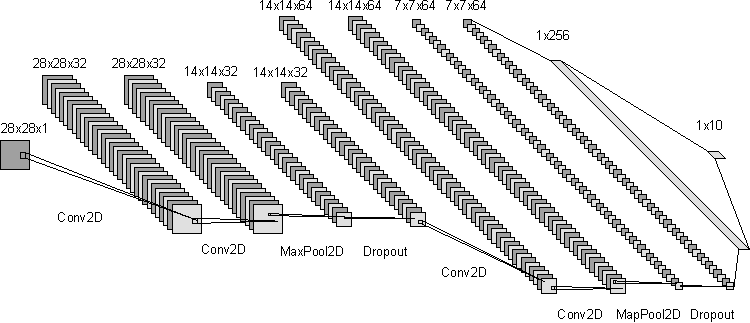
\includegraphics[width=\textwidth]{resources/pdf/ghouzam.pdf}
        \caption{Ghouzam neural network model.}
    \end{figure}
\end{frame}

\begin{frame}{Pre-Trained Models}
    \begin{itemize}
        \item VGG16
        \item MobileNet
        \item ResNet164
    \end{itemize}
\end{frame}

\begin{frame}{VGG16}
    \begin{figure}
        \centering
        \includegraphics[scale=0.6]{resources/png/VGG16.png}
        \caption{VGG16 structure. \footnotemark}
        \label{fig:my_label}
    \end{figure}
    \footnotetext{https://www.quora.com/How-does-VGG-network-architecture-work}
\end{frame}

\begin{frame}{MobileNet}
    \begin{columns}
        \column{0.45\textwidth}
        \begin{figure}
            \centering
            \includegraphics[width=1\textwidth]{resources/png/NormalConvolution.PNG}
            \caption{Normal convolution.\footnotemark}
        \end{figure}
        \column{0.55\textwidth}
        \begin{figure}
            \centering
            \includegraphics[width=1\textwidth]{resources/png/MobileNet.PNG}
            \caption{Depth-wise convolution.\footnotemark[2]}
        \end{figure}
    \end{columns}
\footnotetext{https://machinethink.net/blog/googles-mobile-net-architecture-on-iphone/}
\end{frame}

\begin{frame}{ResNet164}
    \begin{figure}
        \centering
        \includegraphics[scale = 0.45]{resources/png/SkipConnections.PNG}
        \caption{Skip connections in ResNet models.\footnotemark}
    \end{figure}
    \footnotetext{https://cv-tricks.com/keras/understand-implement-resnets/}
\end{frame}

\section{Performance evaluation}

\begin{frame}{Performance Criteria}
    \begin{itemize}
        \item \textbf{Accuracy} : Proportion of cells that were correctly identified.
        \item \textbf{Non-zero Accuracy} : Proportion of non-empty cells that were correctly identified.
        \item \textbf{Confusion matrix} : For the overall accuracy.
    \end{itemize}
\end{frame}

\begin{frame}{Ghouzam}
    \only<1>{
        \textbf{Accuracy} : \num{0.976} \\
        \textbf{Non-zero accuracy} : \num{0.957}
        \begin{center}
            \includegraphics[width=0.8\textwidth]{resources/png/ghouzam_confusion.png}
        \end{center}
    }
    \only<2>{
        Empty cells are not always detected as such.
        \begin{center}
            \includegraphics[width=0.8\textwidth]{resources/png/ghouzam_confusion_empty.jpg}
        \end{center}
    }
    \only<3>{
        Empty cells are not always detected as such.
        \vspace{1em}
        \begin{columns}
            \column{0.5\textwidth}
            \centering
            \includegraphics[width=0.9\textwidth]{resources/png/surimpression1.png}
            \column{0.5\textwidth}
            \centering
            \includegraphics[width=0.9\textwidth]{resources/png/surimpression2.png}
        \end{columns}
    }
    \only<4>{
        Confusion between 1 and 7.
        \begin{center}
            \includegraphics[width=0.8\textwidth]{resources/png/ghouzam_confusion_1_7.jpg}
        \end{center}
    }
    \only<5>{
        Confusion between 1 and 7.
        \vspace{0.5em}
        \begin{columns}
            \column{0.6\textwidth}
            \includegraphics[width=\textwidth]{resources/png/MNIST.png}
            \column{0.4\textwidth}
            \includegraphics[width=\textwidth]{resources/png/1_7.png}
        \end{columns}
        \vspace{0.5em}
        \footnotetext{https://www.kaggle.com/oddrationale/mnist-in-csv}
    }
    \only<6>{
        Handwritten digits (1877 digits) : accuracy of \num{0.882}.
        \begin{center}
            \includegraphics[width=0.66\textwidth]{resources/png/confusion_hand.png}
        \end{center}
        \begin{center}
            \includegraphics[width=0.66\textwidth]{resources/png/handwritten.png}
        \end{center}
    }
    \only<7>{
        Typewritten digits (15497 digits) : accuracy of \num{0.984}.
        \begin{center}
            \includegraphics[width=0.66\textwidth]{resources/png/confusion_type.png}
        \end{center}
        \begin{center}
            \includegraphics[width=0.66\textwidth]{resources/png/type_agg.png}
        \end{center}
    }
\end{frame}

\begin{frame}{Pre-trained models}
    \begin{columns}
        \column{0.55\textwidth}
        \begin{figure}
            \centering
            \includegraphics[width=1\linewidth]{resources/png/ResNet164_ConfusionMatrix.PNG}
            \caption{Confusion matrix for the ResNet164 model}
        \end{figure}
        \column{0.45\textwidth}
        \begin{itemize}
            \item Confusion between all numbers and empty cells
            \item \textbf{Accuracy :} 0.692\\
            (0.327 for VGG16, and 0.424 for MobileNet)
            \item \textbf{Non-zero Accuracy :} 0.442
            (0.323 for VGG16, and 0.420 for MobileNet)
        \end{itemize}
    \end{columns}
\end{frame}

\begin{frame}{Pre-Trained models : Example}
    \centering
    \includegraphics[scale = 0.4]{resources/png/ResnetOverlay.jpg}
\end{frame}

\begin{frame}{Pre-trained models}
    \textbf{Main issues :}
    \begin{itemize}
        \item No empty cells in mnist
        \item Shape of the ones in mnist
        \item Augmented training set
        \item probability threshold
    \end{itemize}
\end{frame}

%%%%%%%%%%%%%%%%%%%%%%%%%
%%%%% Demonstration %%%%%
%%%%%%%%%%%%%%%%%%%%%%%%%

\begin{frame}[standout]
    Demonstration
\end{frame}

\end{document}
